% Chapter 4
\newpage
\begingroup%
\makeatletter%
\let\clearpage\relax% Stop LaTeX from going to a new page; and
\vspace*{\fill}%
\vspace*{\dimexpr-50\p@-\baselineskip}% Remove the initial (default) 50pt gap (plus 1 line)
\chapterfont{\centering}
\chapter{Implementation} % Write in your own chapter title

\vspace*{\fill}%
\endgroup

\newpage
\label{Chapter4}
\lhead{Chapter 4. \emph{Implementation}} % Write in your own chapter title to set the page header


\section{Implementation Details}
The system consists of different modules like an E-commerce website, a 3D tour of a MetaMart store, Virtual reality mode, and fitting size suggestions for customers. These are the main modules of our web application.
The implementation detail of each of the following modules is discussed in detail below.
\section{Rules and assumptions}
Following are rules and cases of assumptions that are assumed to be true while experiencing virtual reality mode working:
\begin{itemize}
    \item The customer has an Oculus VR headset and the configurations/setting for Oculus VR Headset is also done by the customer before going into VR mode.
\end{itemize}
Following are rules and cases of assumptions that are assumed to be true while normally working:
\begin{itemize}
    \item The internet connection is stable.
\end{itemize}
\section{Technology Used}
\subsection{Frontend}
Following are the languages we used in this project:
\begin{itemize}
  \item HTML5
  \item CSS
  \item Bootstrap5
  \item JavaScript
  \item React
  \item NodeJs
  \item Redux
\end{itemize}  
\subsection{Database}
We used  \textbf{MongoDb} database which is one of the popular NoSQL databases.We used mongodb with NodeJs.\\ We also used express as it is also one of the popular backend frameworks for node.
\subsection{API}
Express.Js: It is an open source for node js used to integrate frontend
and backend.

\section{System Requirement}

To be able to use certain hardware or software, the system requirements are required specifications. The configurations for VR headsets are necessary so that the VR headset will work fine and the customer can experience virtual reality mode without any problems. A computer may need certain input and output ports to work with peripheral devices. So as our application requires a VR headset with its configurations on the system, that's why ports should work fine because different cables i.HDMI cables need to be inserted into respective ports.
\subsection{Hardware Requirement}
Following are some of the hardware requirements for this project:
\begin{itemize}
   \item Processor Intel(R)  
    \item Installed RAM 8.00GB
    \item Window 8,10,11
    \item Wireless Adapter(WIFI) or Ethernet connections(LAN)
    \item Oculus VR Headset( For experiencing Virtual reality-based E-commerce store)
\end{itemize}
 
\subsection{Software Requirement}
\begin{itemize}
    \item Software Stack: MERN 
    \item IDE: Visual Studio
    \item Database: MongoDB
    \item Testing API: Postman
\end{itemize}
\section{Tools Used}
A list of all the software that is used to develop and needed to operate the developed module is detailed below:
\begin{table}[H]
    \centering
   \begin{tabular}{ | m{7em} | m{11cm}|}  
  \hline  \textbf{Tools} &  \textbf{Description}  \\  \hline
 \textbf{Make-Human} & MakeHuman is a free and open-source application used for making 3D avatars with custom inputs. Like we just have to set input measurements for the avatars. We can also import and export avatars. Make-Human is developed by a community of programmers.
  \\  \hline
 \textbf{Clo3D} & Clo3D enables you to create virtual 3D samples using best practices and workflow and provides you with basic knowledge of pattern making and digital pattern files. You learn how to instantly modify patterns, fit, and fabrication, with the ability to view changes in colors, prints, and graphics. We can easily make 3D clothes using clo3D.
    \\  \hline
\textbf{ Balsamiq} & Balsamiq Cloud is a web-based user interface design tool for creating wireframes. It can be used to generate digital sketches of your idea or concept for an application or website and to facilitate discussion and understanding before any code is written. You can use Balsamiq to make wireframes. We can make low-fidelity prototypes of our application.
    \\  \hline
 \textbf{ Asana} & Asana is a web and mobile work management platform designed to help teams and organizations organize, track, and manage their tasks or work. 
    \\  \hline
 \textbf{ Github} & GitHub is an online software development platform. It's used for storing, tracking, and collaborating on software projects.GitHub is a great platform for source code sharing and tracking changes in it. With the help of Github, you can easily share your source code with another person.
    \\  \hline
   \textbf{ VS Code} & With VS Code, a free coding editor, you can quickly begin coding.Use it to code in any programming language, without switching editors.
        \\  \hline
    \textbf{Overleaf} & Overleaf is a collaborative cloud-based LaTeX editor used for writing, editing, and publishing scientific documents.
    \\  \hline
    \textbf{Visual Studio} & You can get started coding right away with the help of the free coding editor Visual Studio Code. Visual Studio Code has support for many programming languages, including Python, Java, C++, JavaScript, and many more.
    \\  \hline
    \textbf{  Zoom} & Zoom is a communication Platform. You can use it for users to connect with video, audio, phone, and chat.
       \\  \hline
    \textbf{Postman} & Postman is an API platform for building and using APIs. Postman simplifies each step of the API lifecycle and streamlines collaboration so you can create better APIs—faster.
    \\  \hline
\end{tabular}
    \caption{Tools required for the development of proposed system}
    \label{tab: Tools required for the development of proposed system}
\end{table}
The given table shows the list of different tools that are going to be used for the proposed system’s development. For example, in the first place, there is a tool named “make human”. This tool would be helping out developers in making 3D avatars by giving custom measurements (height, weight, chest size, arm size e.t.c) to the application and getting avatars of that size as output.  Similarly, clo3d will be used for making 3D clothes models to give customers 360-degree exposure. 
\section{3D Jackets View}
\subsection{For Males}
\begin{figure}[H]
    \centering
    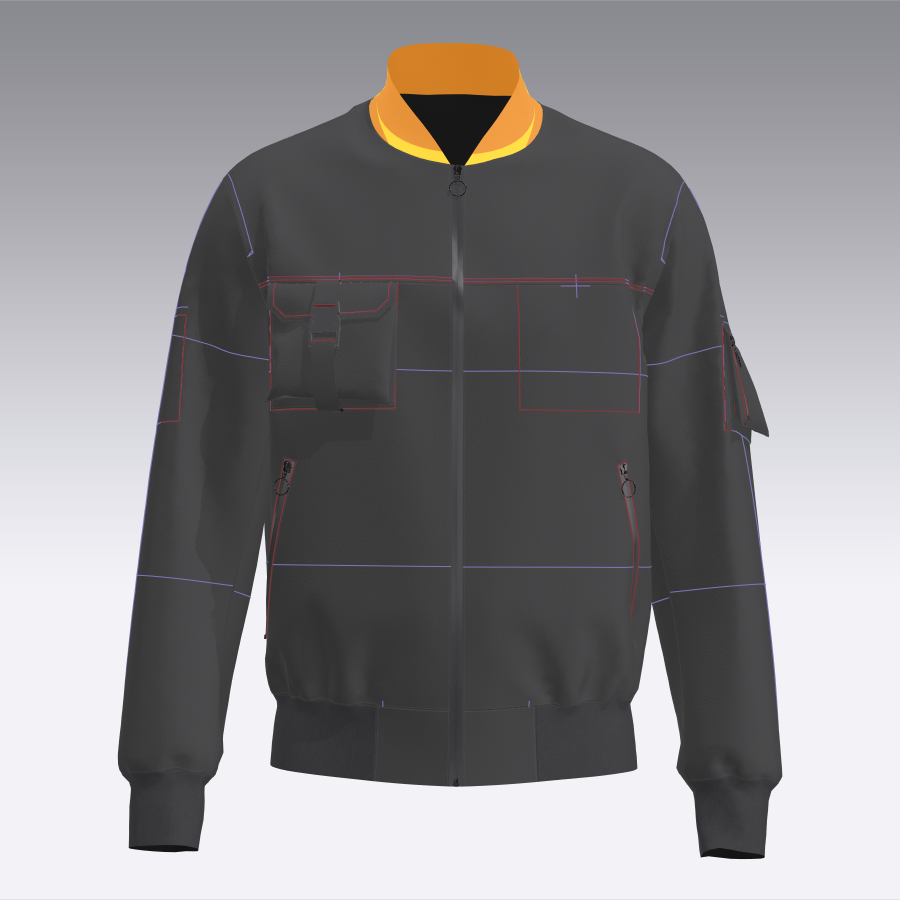
\includegraphics[width=13cm,height=13cm]{Figures/3DJackets/male1.png}
    \caption{3D Model of the grey jacket (Male)}
    \label{fig1:3D Model of the grey jacket (Male)}
   
\end{figure}
\justifying
 A 3D model of a grey color jacket for men made in clo3d. The purpose of this model is to put it on the avatar and render it as a 360-degree rotatable object for customers in 3D environment. This jacket is made by making some patterns and then sewing that patterns according to some measurements.
\begin{figure}[H]
    \centering
    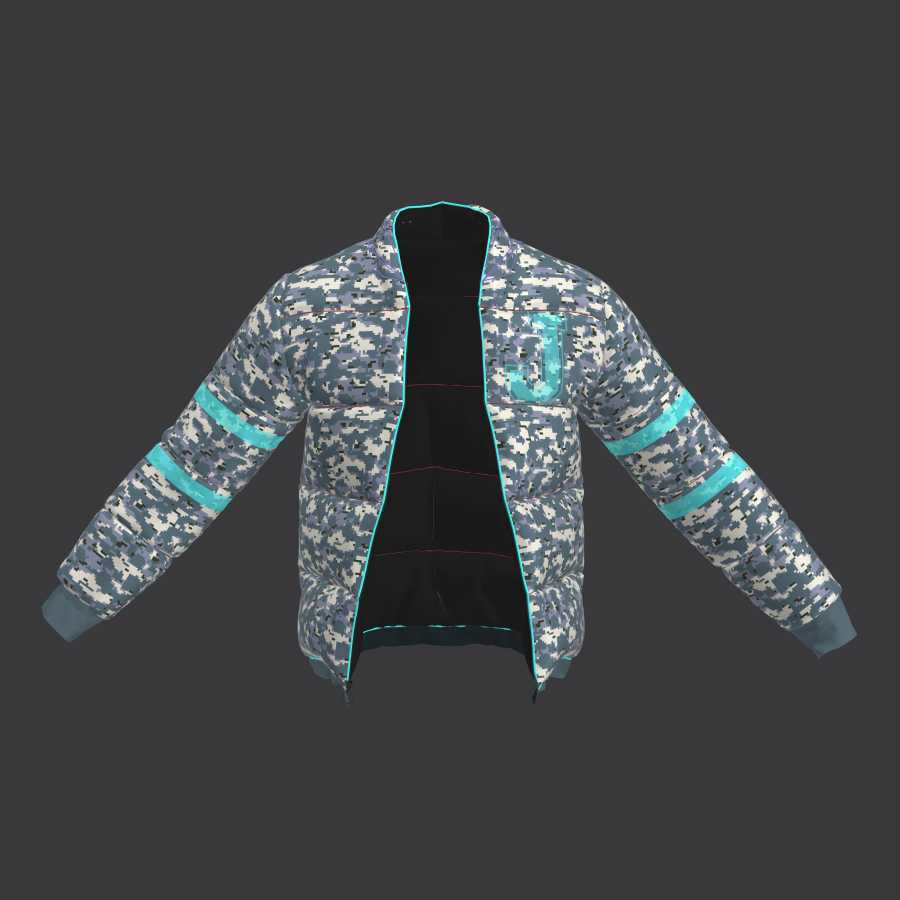
\includegraphics[width=13cm,height=13cm]{Figures/3DJackets/male2.png}
    \caption{3D Model of the jacket (Male)}
    \label{fig2:3D Model of the jacket (Male)}

\end{figure}
\justifying
A 3D model of khaaki color jacket for men made in clo3d. The purpose of this model is to put it on an avatar and render it as a 360-degree rotatable object for customers in a 3D environment. This jacket is made by making some patterns and then sewing that patterns according to some measurements.
\begin{figure}[H]
    \centering
    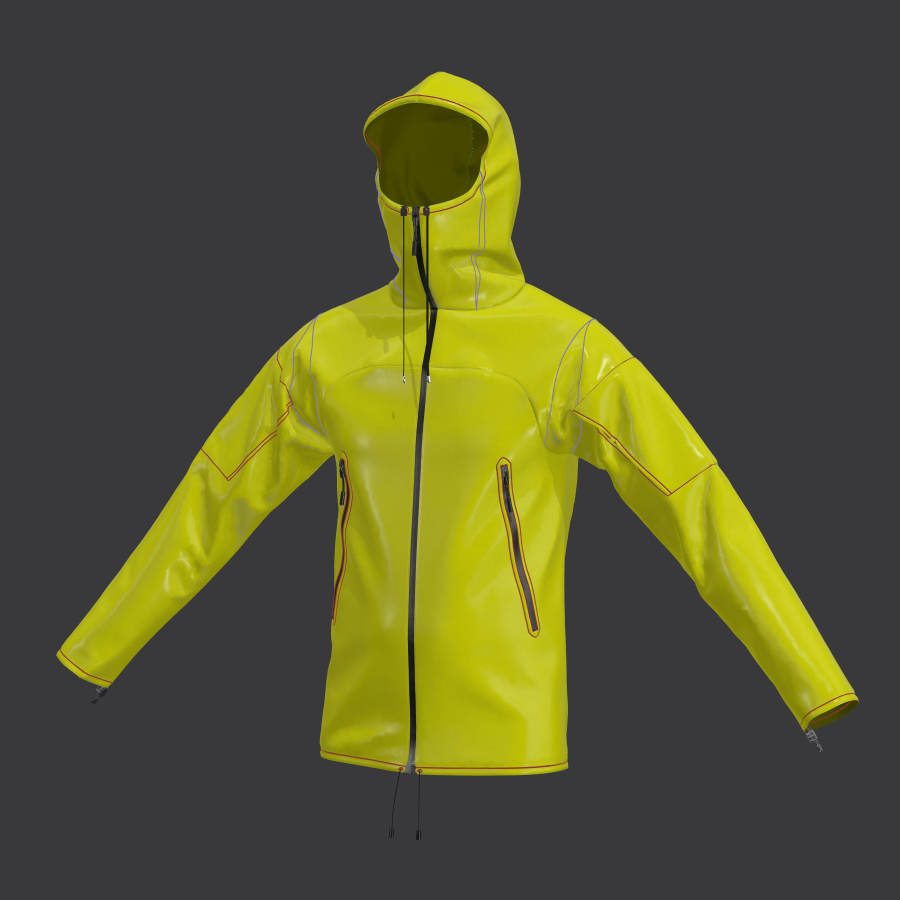
\includegraphics[width=13cm,height=13cm]{Figures/3DJackets/male3.png}
    \caption{3D Model of the yellow jacket (Male)}
    \label{fig3:3D Model of the yellow jacket (Male)}
\end{figure}
\justifying
A 3D model of a yellow color jacket for men made in clo3d. The purpose of this model is to put it on the avatar and render it as a 360-degree rotatable object for customers in a 3D environment. This jacket is made by making some patterns and then sewing that patterns according to some measurements.
\begin{figure}[H]
    \centering
    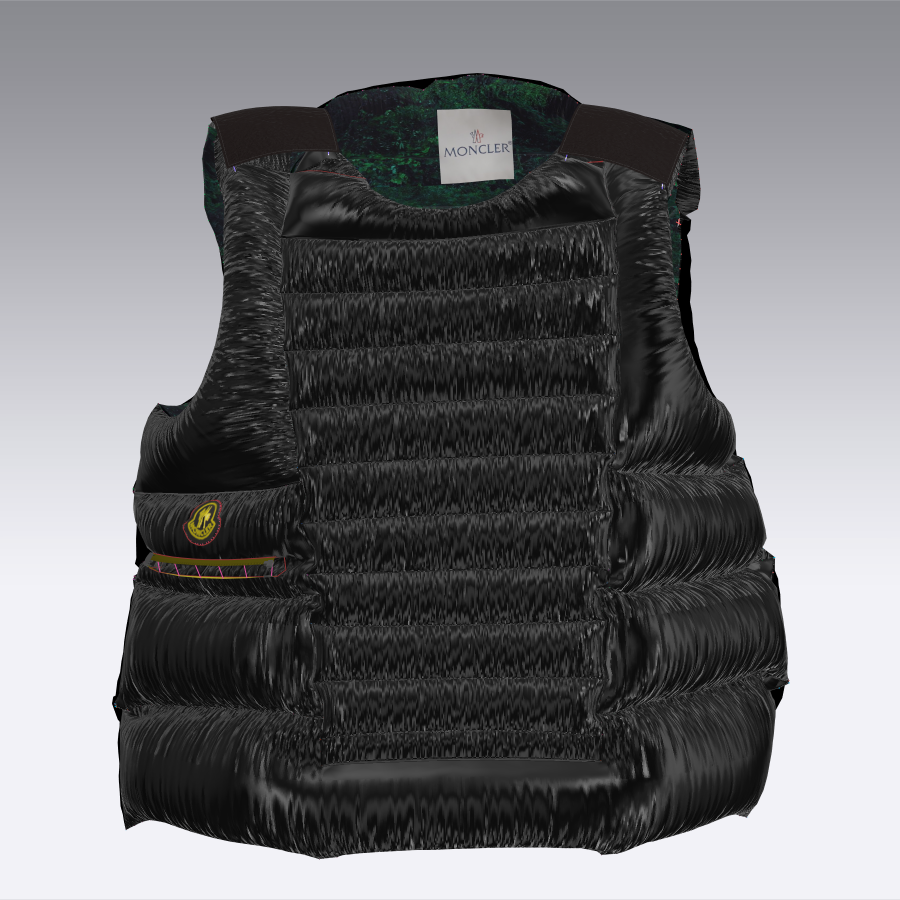
\includegraphics[width=13cm,height=13cm]{Figures/3DJackets/male4.png}
    \caption{3D Model of sleeveless black puffer jacket (Male)}
    \label{fig4:3D Model of sleeveless black puffer jacket (Male)}
  
\end{figure}
\justifying
A 3D model of black color puffer jacket for men made in clo3d. The purpose of this model is to put it on the avatar and render it as a 360-degree rotatable object for customers in a 3D environment. This jacket is made by making some patterns and then sewing that patterns according to some measurements.
\begin{figure}[H]
    \centering
    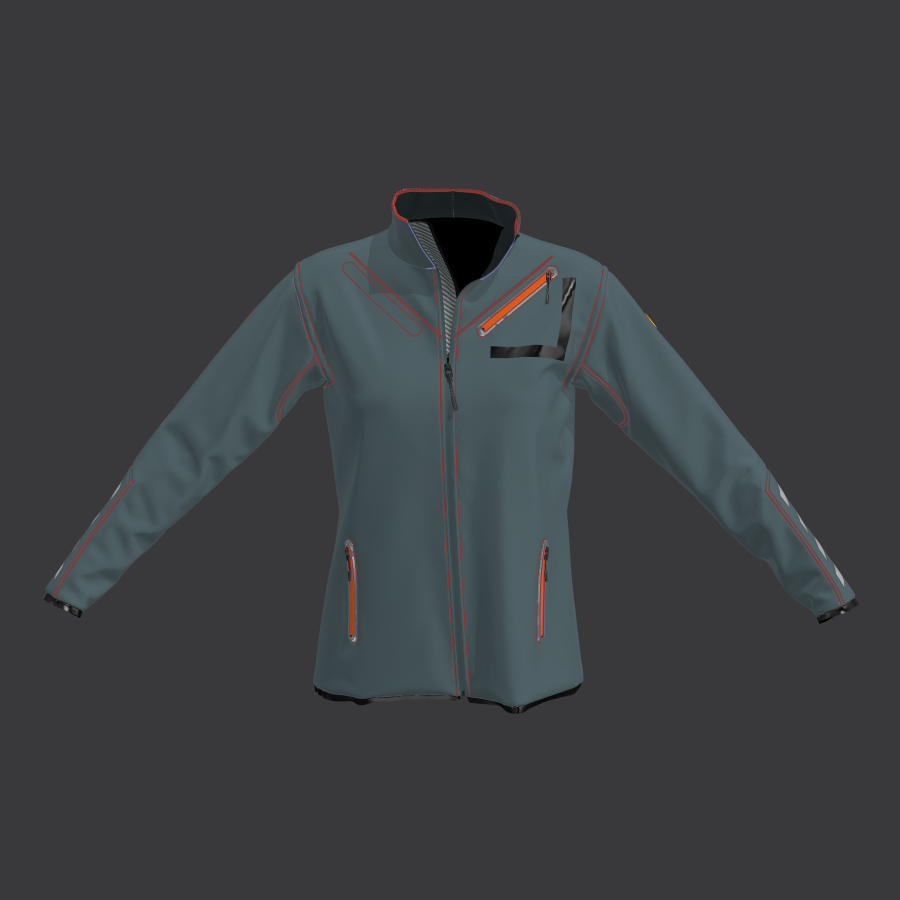
\includegraphics[width=15cm,height=15cm]{Figures/3DJackets/male5.png}
    \caption{3D Model of the jacket (Male)}
    \label{fig5:3D Model of the jacket (Male)}
\end{figure}
\justifying
A 3D model of a jacket for men made in clo3d. The purpose of this model is to put it on the avatar and render it as a 360-degree rotatable object for customers in a 3D environment. This jacket is made by making some patterns and then sewing that patterns according to some measurements.
\subsection{For Females}
\begin{figure}[H]
    \centering
    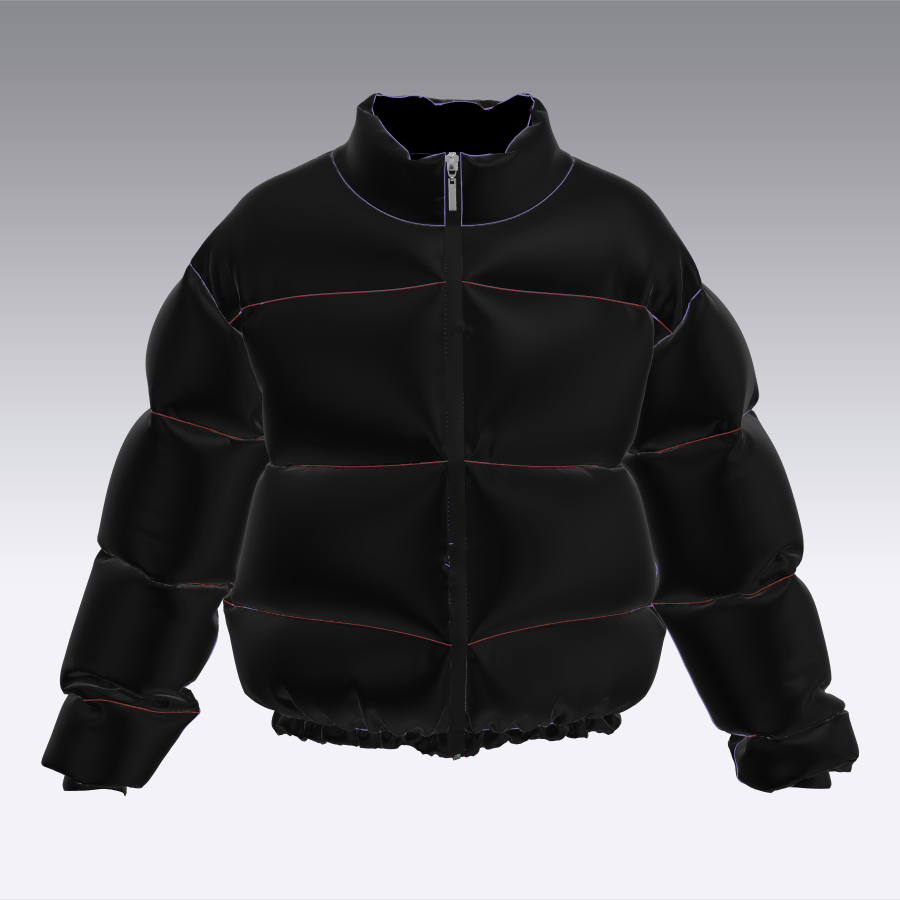
\includegraphics[width=13cm,height=12cm]{Figures/3DJackets/female1.png}
    \caption{3D Model of puffer jacket (Female)}
    \label{fig1:3D Model of puffer jacket (Female)}
\end{figure}
\justifying
A 3D model of a black color jacket for females. The purpose of this model is to put it on the avatar and render it as a 360-degree rotatable object for customers in a 3D environment. This jacket is made by making some patterns and then sewing that patterns according to some measurements.
\begin{figure}[H]
    \centering
    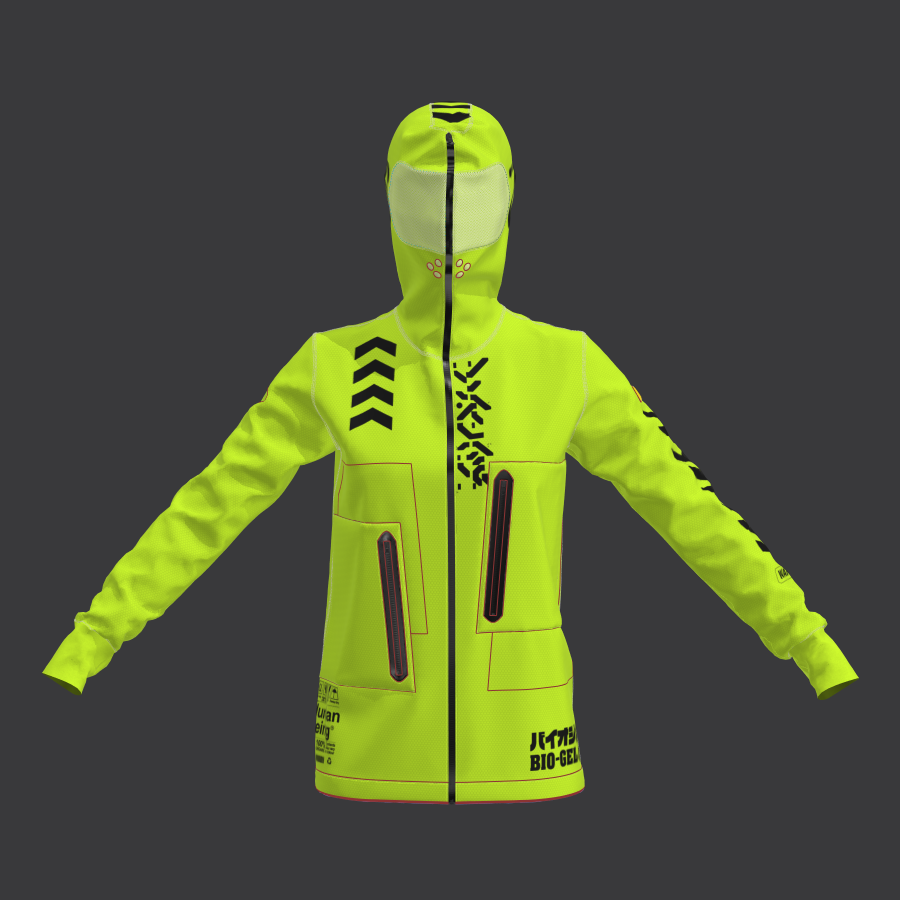
\includegraphics[width=13cm,height=12cm]{Figures/3DJackets/female2.png}
    \caption{3D Model of the stylish designed jacket (Female)}
    \label{3D Model of the stylish designed jacket (Female)}

\end{figure}
A 3D model of a well-designed jacket for females. The purpose of this model is to put it on the avatar and render it as a 360-degree rotatable object for customers in a 3D environment. This jacket is made by making some patterns and then sewing that patterns according to some measurements.
\begin{figure}[H]
    \centering
    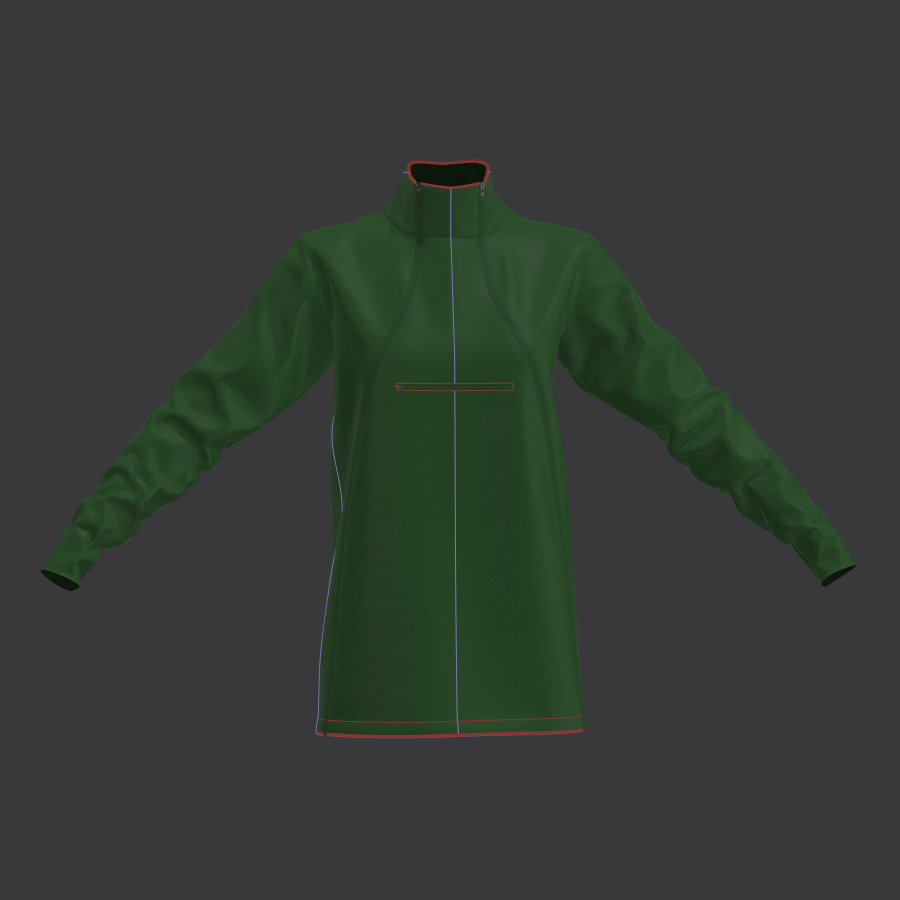
\includegraphics[width=13cm,height=12cm]{Figures/3DJackets/female3.png}
    \caption{3D Model of the green leather jacket (Female)}
    \label{3D Model of the green leather jacket (Female)}
   
\end{figure}
A 3D model of a well-designed leather jacket for females. The purpose of this model is to put it on the avatar and render it as a 360-degree rotatable object for customers in the 3D environment. This jacket is made by making some patterns and then sewing that patterns according to some measurements.
\begin{figure}[H]
    \centering
    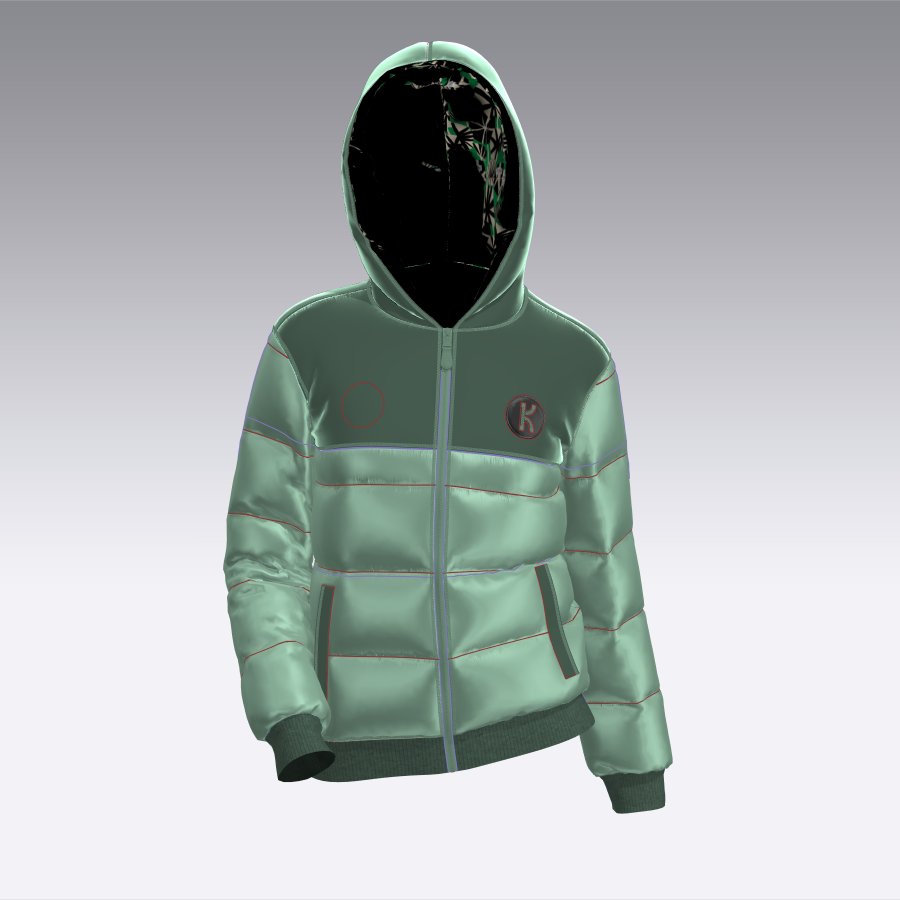
\includegraphics[width=13cm,height=12cm]{Figures/3DJackets/female4.png}
    \caption{3D Model of beautifully designed puffer jacket (Female)}
    \label{3D Model of beautifully designed puffer jacket (Female)}
  
\end{figure}
\justifying
A 3D model of a well-designed puffer jacket for females. The purpose of this model is to put it on the avatar and render it as a 360-degree rotatable object for customers in a 3D environment. This jacket is made by making some patterns and then sewing that patterns according to some measurements.
\section{3D Avatars wearing Jackets View}
\subsection{For Males}
\begin{figure}[H]
    \centering
    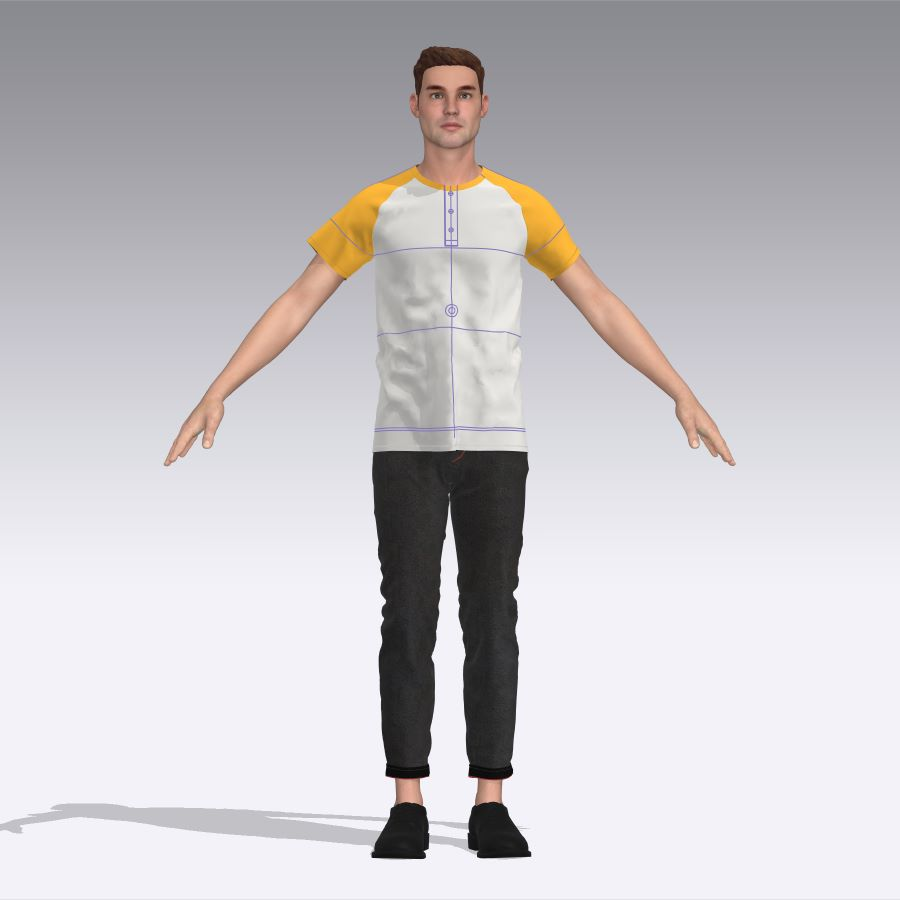
\includegraphics[width=13cm,height=12cm]{Figures/3DAvatars/male1.jpeg}
    \caption{Male Avatar wearing t-shirt and pants}
    \label{Male Avatar wearing t-shirt and pants}
   
\end{figure}
	Avatar is a 3D rotatable object made in make humans with customer inputs. It would be used for displaying 3D clothes to the customer just like in the real world there are statues for displaying clothes and customers can move around that statue for checking cloth.  
\begin{figure}[H]
    \centering
    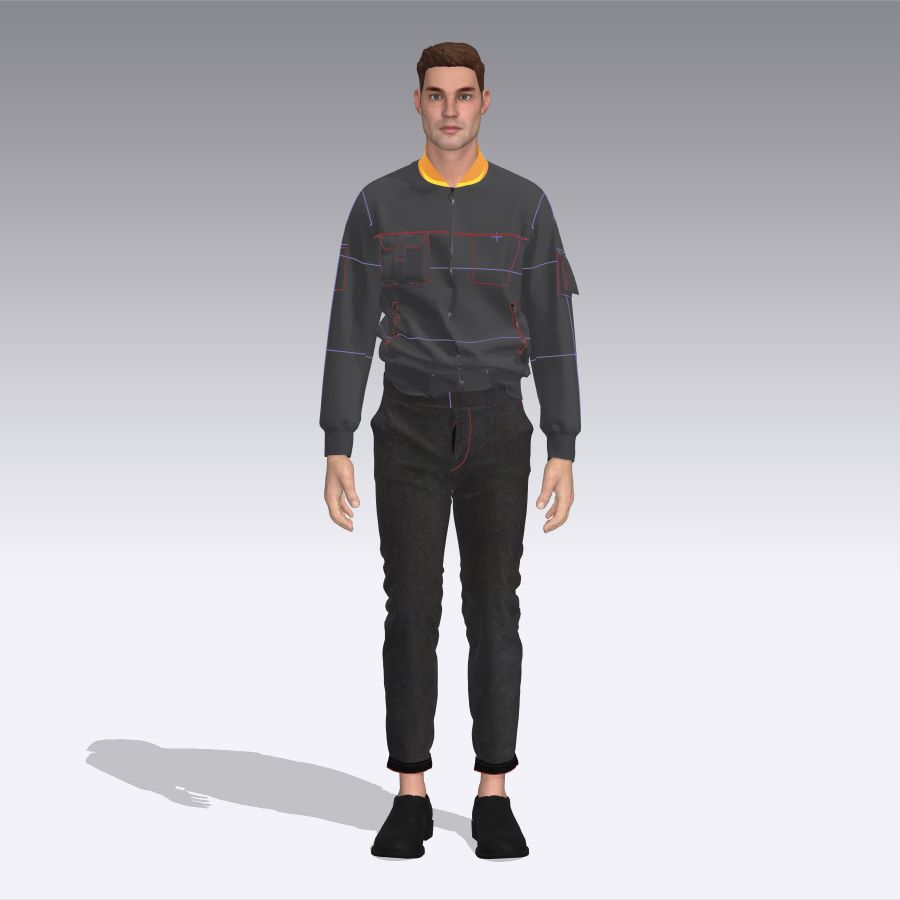
\includegraphics[width=12cm,height=10cm]{Figures/3DAvatars/male2.jpeg}
    \caption{Male Avatar wearing jacket and pants}
    \label{Male Avatar wearing jacket and pants}
 
\end{figure}
Avatar is a 3D rotatable object made in make humans with customer inputs. It would be used for displaying 3D clothes to the customer just like in the real world there are statues for displaying clothes and customers can move around that statue for checking cloth.  
\begin{figure}[H]
    \centering
    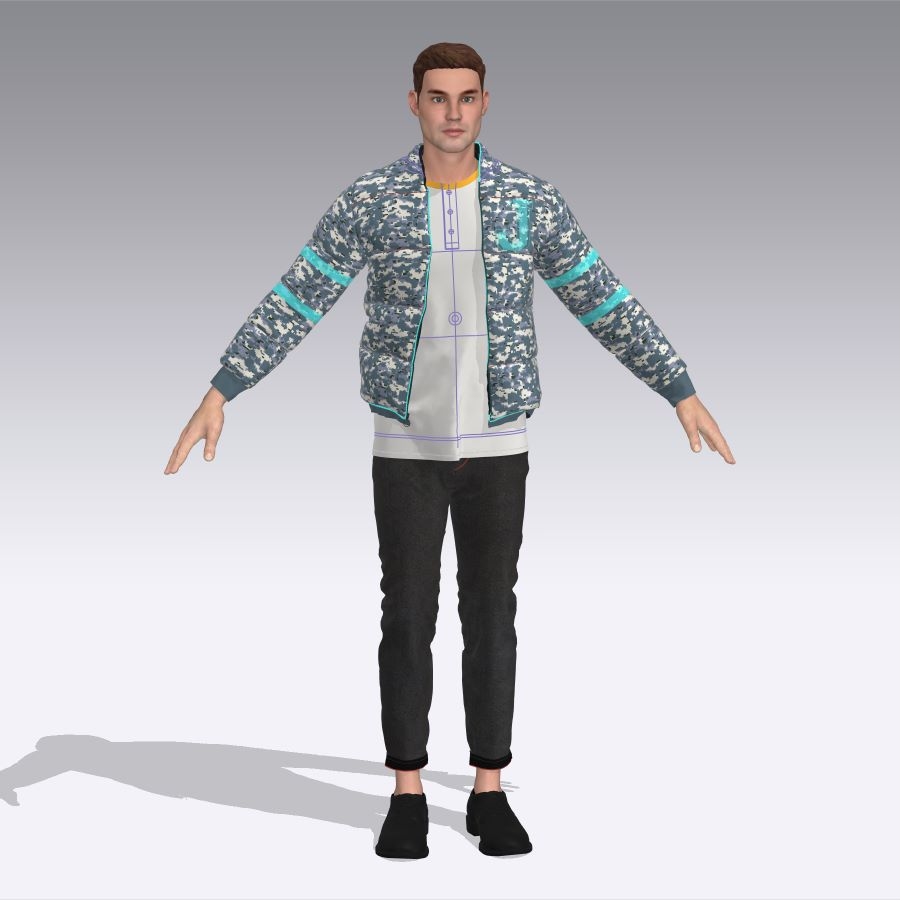
\includegraphics[width=13cm,height=10cm]{Figures/3DAvatars/male3.jpeg}
    \caption{Asian Male Avatar wearing jacket and pants}
    \label{Male Avatar wearing jacket and pants}
    
\end{figure}
Avatar is a 3D rotatable object made in make humans with customer inputs. It would be used for displaying 3D clothes to the customer just like in the real world there are statues for displaying clothes and customers can move around that statue for checking cloth.  
\begin{figure}[H]
    \centering
    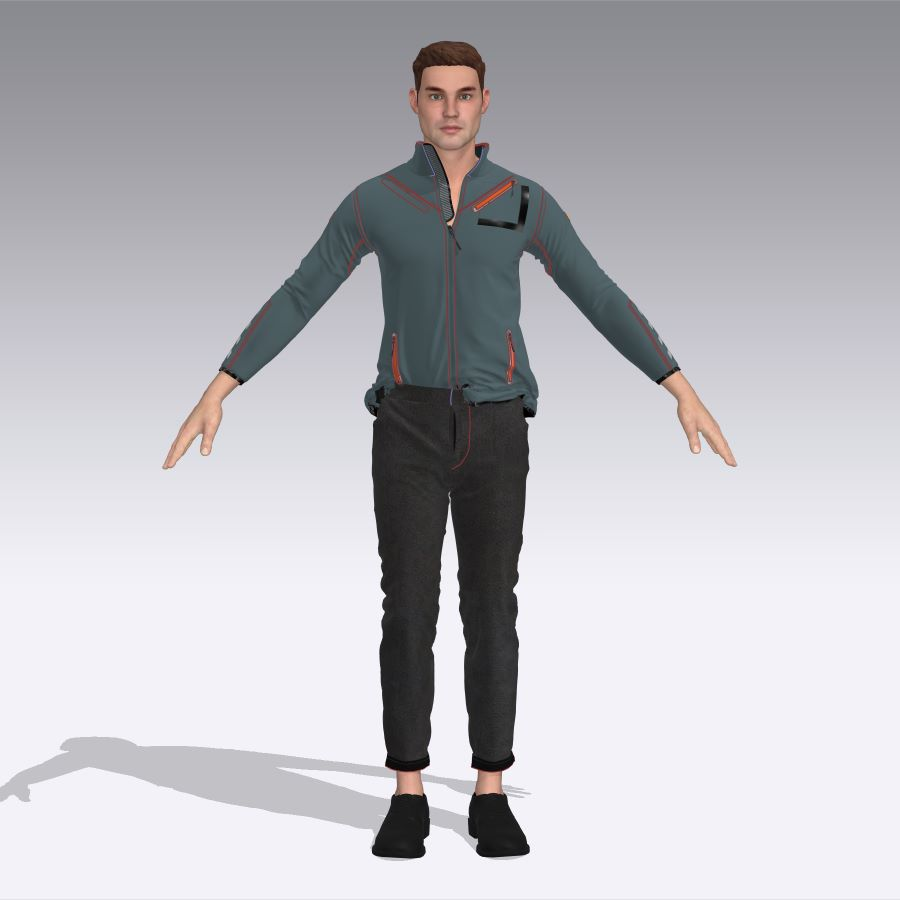
\includegraphics[width=13cm,height=10cm]{Figures/3DAvatars/male4.jpeg}
    \caption{Male Avatar wearing jacket and black pants}
    \label{Male Avatar wearing jacket and black pants}

\end{figure}
\justifying
	Avatar is a 3D rotatable object made in make humans with customer inputs. It would be used for displaying of 3D clothes to the customer just like in the real world there are statues for displaying clothes and customers can move around that statue for checking cloth.  
\subsection{For Females}
\begin{figure}[H]
    \centering
    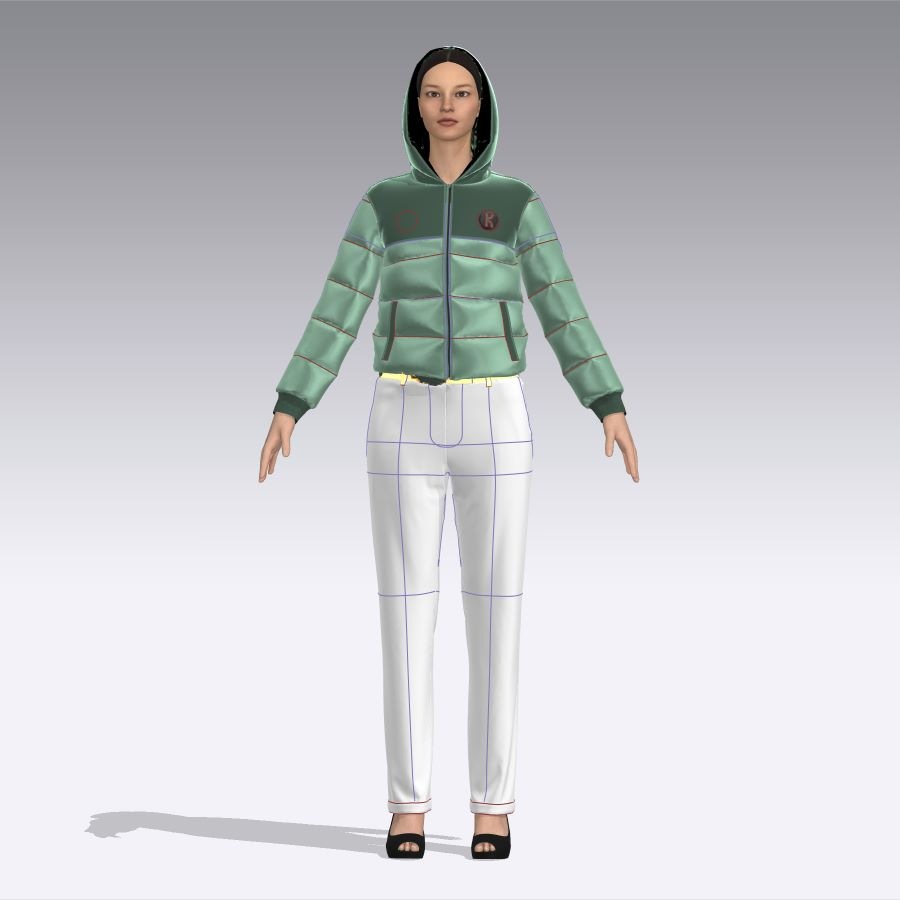
\includegraphics[width=12cm,height=10cm]{Figures/3DAvatars/female1.jpeg}
    \caption{Female Avatar wearing a puffer jacket and white pants}
    \label{Female Avatar wearing a puffer jacket and white pants}
    
\end{figure}
\justifying
Avatar is a 3D rotatable object made in make humans with customer inputs. It would be used for displaying 3D clothes to the customer just like in the real world there are statues for displaying clothes and customers can move around that statue for checking cloth.  


\begin{figure}[H]
    \centering
    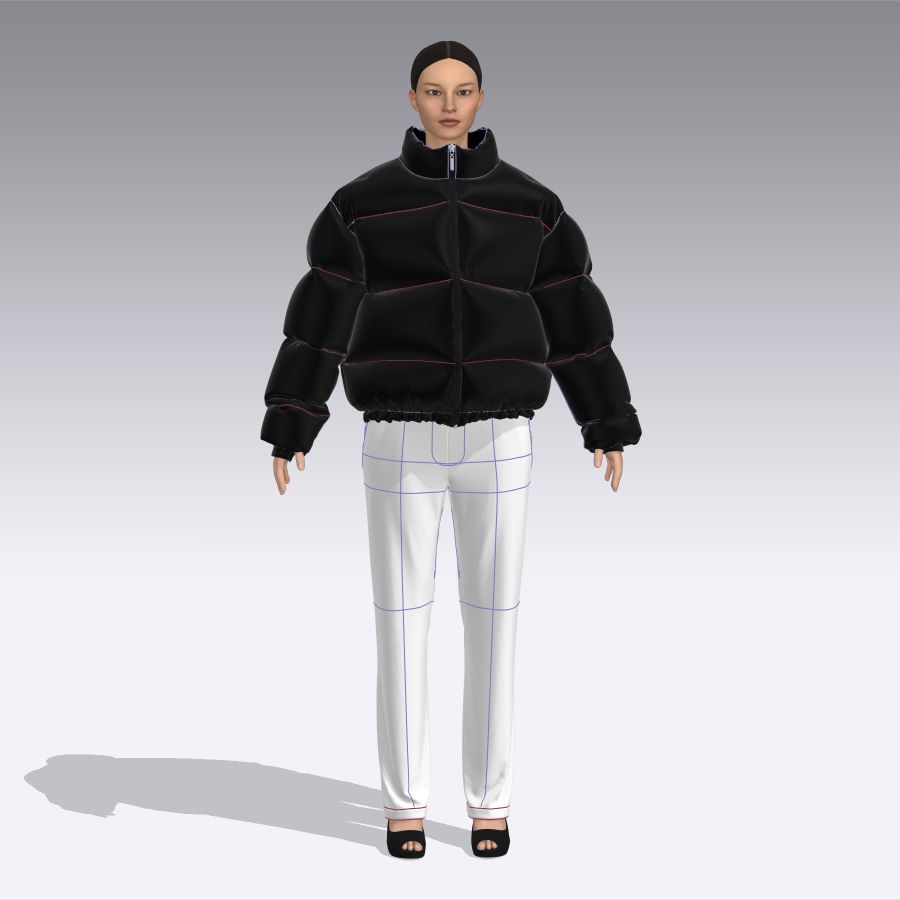
\includegraphics[width=13cm,height=12cm]{Figures/3DAvatars/female2.jpeg}
    \caption{Female Avatar wearing a stylish black puffer jacket and white pants}
    \label{fig2:Stylish designed 3D jacket for females.In this image, you can see the female avatar wearing the jacket. This is the front view.}
\end{figure}
\justifying
	Avatar is a 3D rotatable object made in make humans with customer inputs. It would be used for displaying 3D clothes to the customer just like in the real world there are statues for displaying clothes and customers can move around that statue for checking cloth.  
\section{Unity Environment View}
\subsection{Virtual city in Meta verse}
\begin{figure}[H]
    \centering
    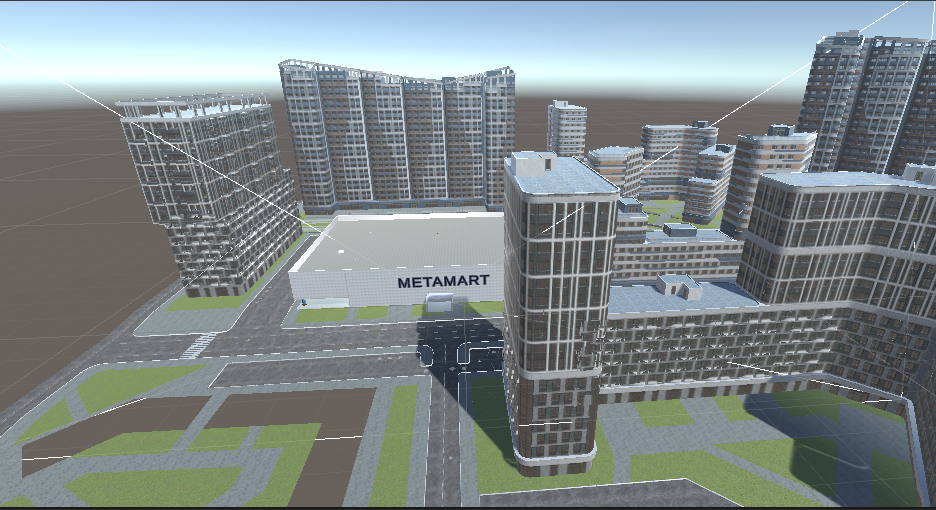
\includegraphics[width=12cm,height=10cm]{Figures/Environment/City.png}
    \caption{Virtual store outer view}
    \label{fig: Virtual store outer view}
\end{figure}
  The virtual store's outer view is shown in this image.
\subsection{Entrance of MetaMart}
\begin{figure}[H]
    \centering
    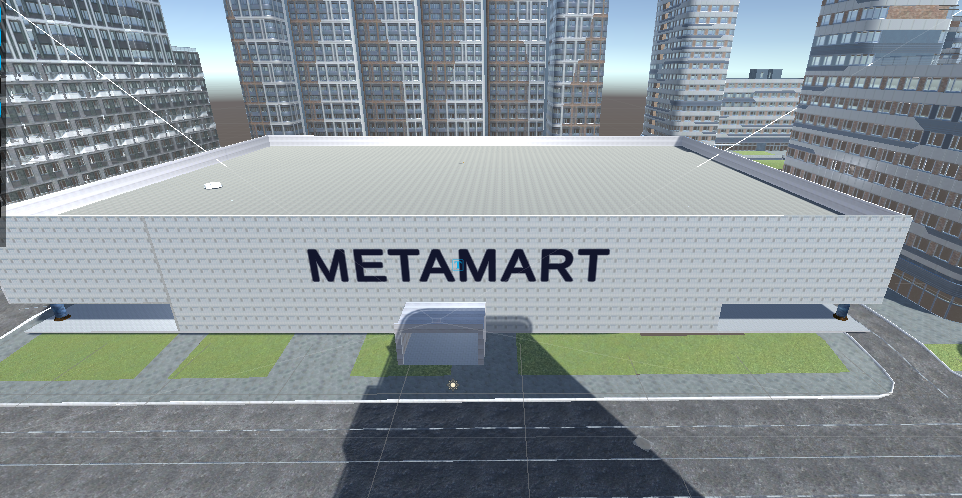
\includegraphics[width=12cm,height=10cm]{Figures/Environment/Entrance.png}
    \caption{Entrance of MetaMart}
    \label{fig: Entrance of MetaMart}
\end{figure}
\justifying
  Entrance of MetaMart through which the customer will enter in the MetaMart.
\subsection{Inside View of MetaMart}
\begin{figure}[H]
    \centering
    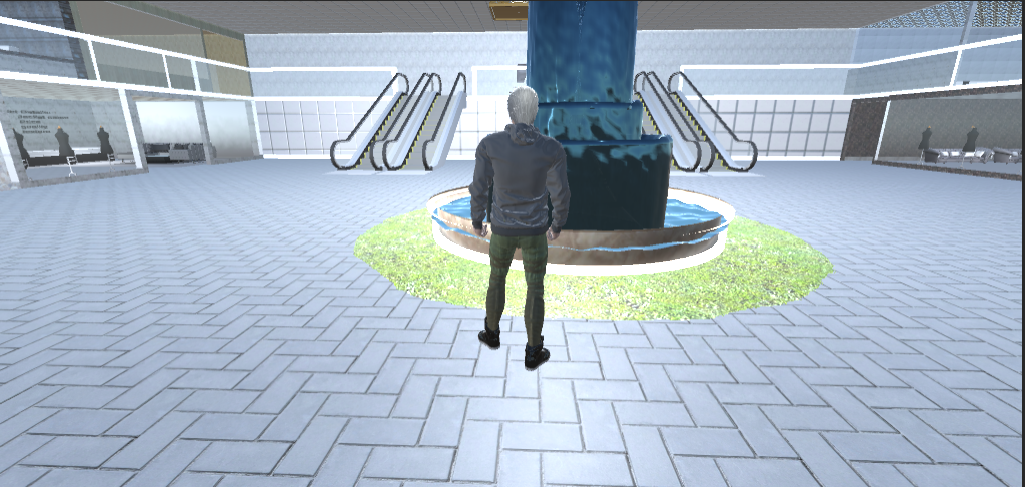
\includegraphics[width=12cm,height=10cm]{Figures/Environment/insideview.png}
    \caption{Inside view of MetaMart}
    \label{fig: Entrance of MetaMart}
    
\end{figure}
The front view of shops in MetaMart is in this image is shown.
\subsection{Inside View of MetaMart}
\begin{figure}[H]
    \centering
    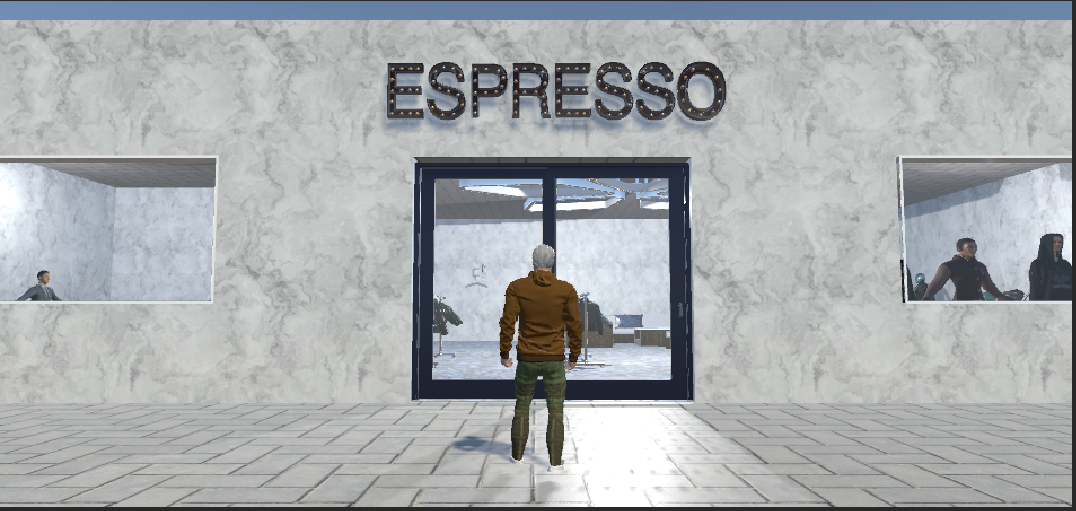
\includegraphics[width=13cm,height=12cm]{Figures/Environment/shop.png}
    \caption{Shop View of MetaMart}
    \label{fig:Shop View of MetaMart}
\end{figure}
The front view of shop in MetaMart in this image is shown.
\subsection{Inside Shop view in MetaMart}
\begin{figure}[H]
    \centering
    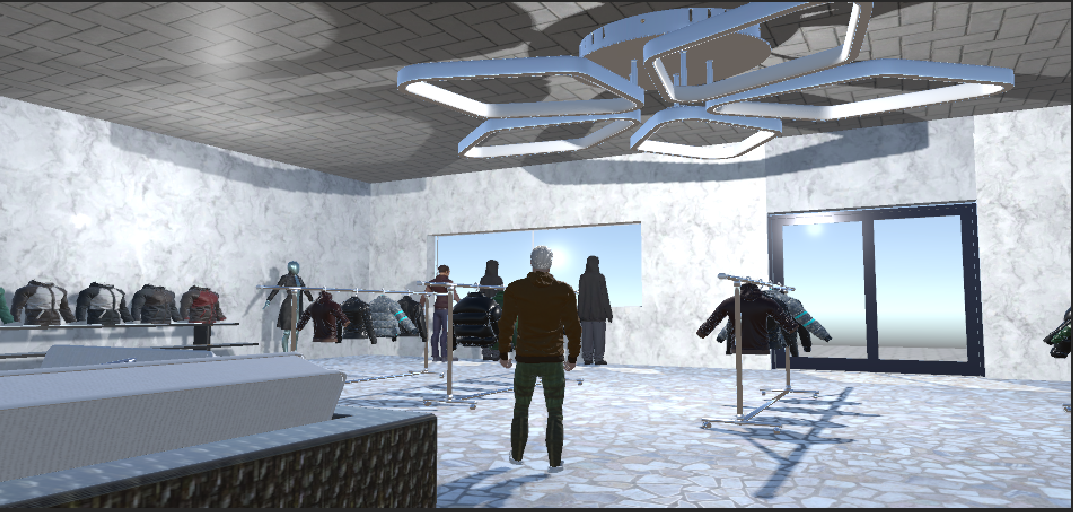
\includegraphics[width=13cm,height=12cm]{Figures/Environment/insideshop.png}
    \caption{Inside View of MetaMart}
    \label{fig:Inside View of MetaMart}
\end{figure}
  Inside View of MetaMart like when the customer enters the shop in MetaMart this view will be shown to the customer.
  \begin{figure}[H]
    \centering
    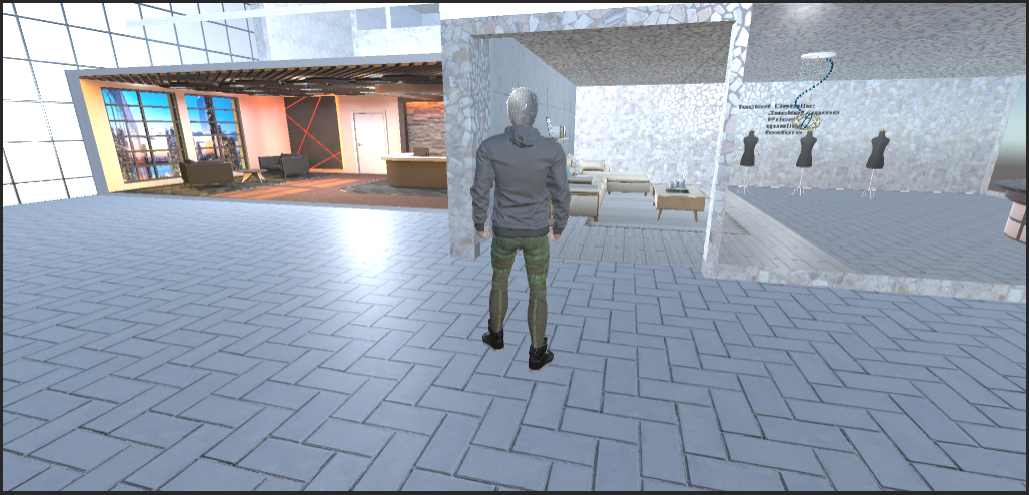
\includegraphics[width=13cm,height=12cm]{Figures/Environment/insideview22.png}
    \caption{Inside View of MetaMart (2)}
    \label{fig:Inside View of MetaMart(2)}
\end{figure}
  Inside View of MetaMart like when the customer enters the shop in MetaMart this view will be shown to the customer.
\begin{figure}[H]
    \centering
    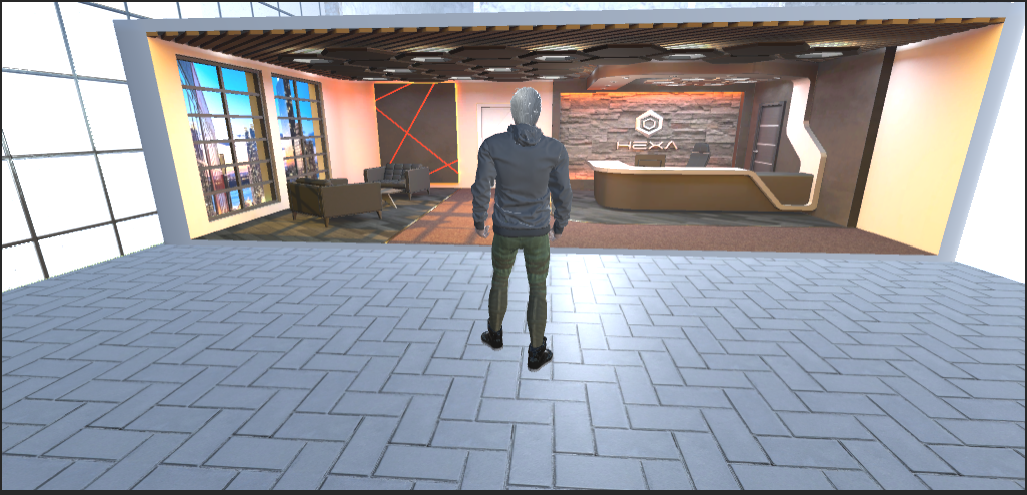
\includegraphics[width=15cm,height=15cm]{Figures/Environment/insidevie2.png}
    \caption{Inside View of MetaMart(2)}
    \label{fig: Entrance of MetaMart}
\end{figure}
\justifying
  There are different shops inside the MetaMart like when the customer enters in the MetaMart this is the first shop in which there will be different outerwears for men.
\begin{figure}[H]
    \centering
    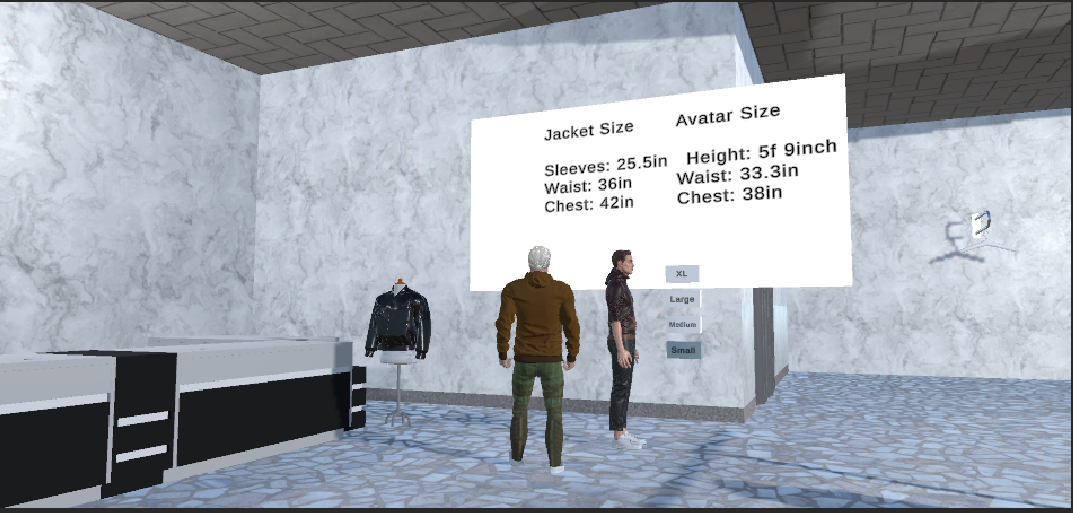
\includegraphics[width=15cm,height=15cm]{Figures/Environment/products.png}
    \caption{Jacket details shown to the customer}
    \label{fig:Product Details showing}
\end{figure}
\justifying
When a customer approaches a product, its details will be displayed to the user, just like this.
\section{Virtual Reality-based E-commerce Web Application Interface}
\subsection{Admin Section}
Following are some of the screenshots of the Admin section:
\subsubsection{Sign-In Screen}
\begin{figure}[H]
    \centering
    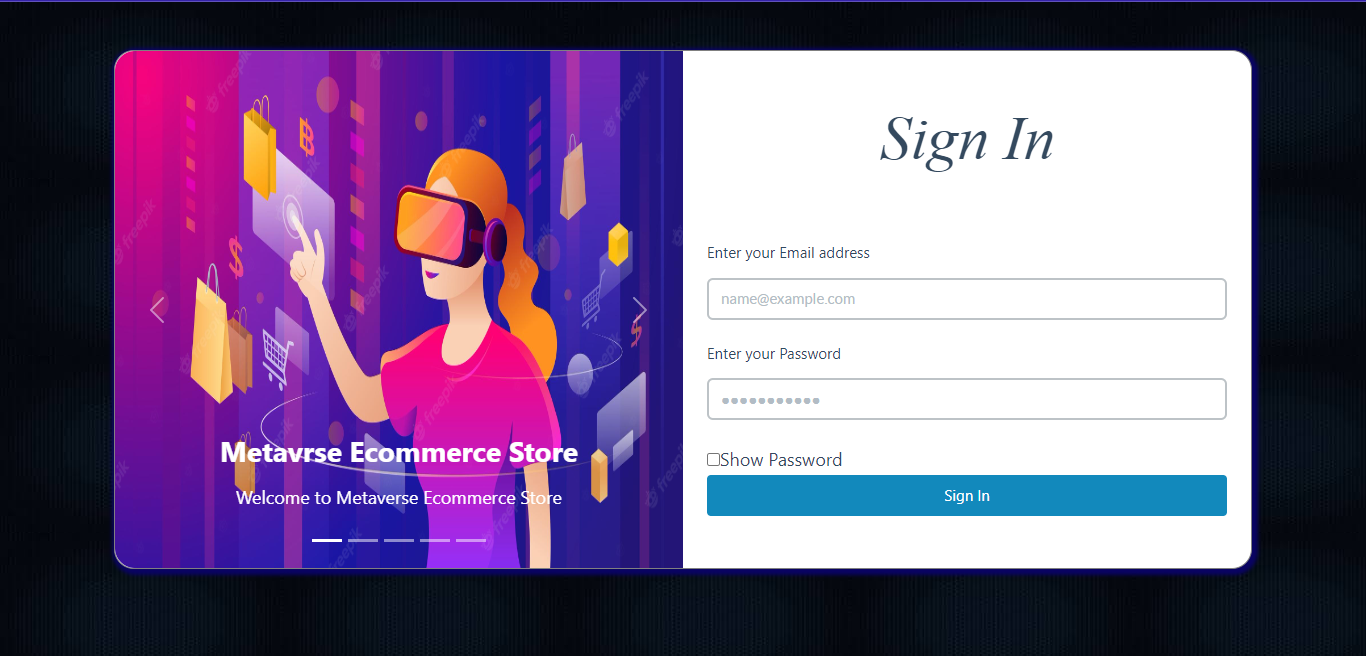
\includegraphics[width=15cm,height=12cm]{Figures/Diagrams/SignIn.PNG}
    \caption{System’s sign-in screen (Admin)}
    \label{System’s sign-in screen (Admin)}
    It is the sign In page for the Admin of the website.
\end{figure}
\justifying
This image shows the sign-in screen that we have developed for our MetaMart Application for admin of the application. On this screen, there is a login form that contains email and password fields. This form is fulfilling all validations.
\subsubsection{Profile Setting Page}
\begin{figure}[H]
    \centering
    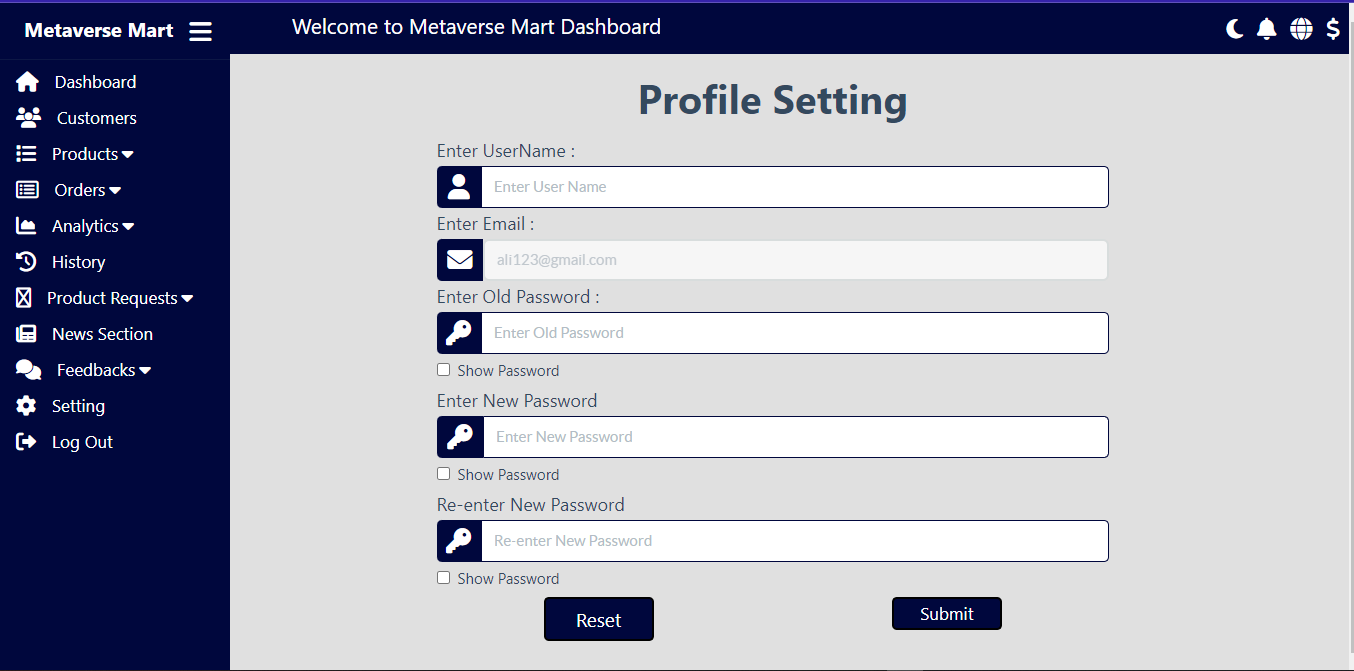
\includegraphics[width=15cm,height=12cm]{Figures/Diagrams/ProfileSetting.PNG}
    \caption{Admin Profile Setting}
    \label{Admin Profile Setting Page}
\end{figure}
\justifying
This image shows the profile setting screen that we have developed for our MetaMart Application for admin of the application. In this screen, there is a form that contains all the fields related to the admin’s profile. This form is fulfilling all validations and valid error messages that would be shown to the user in case of invalid inputs.
\subsubsection{Pending Order}
\begin{figure}[H]
    \centering
    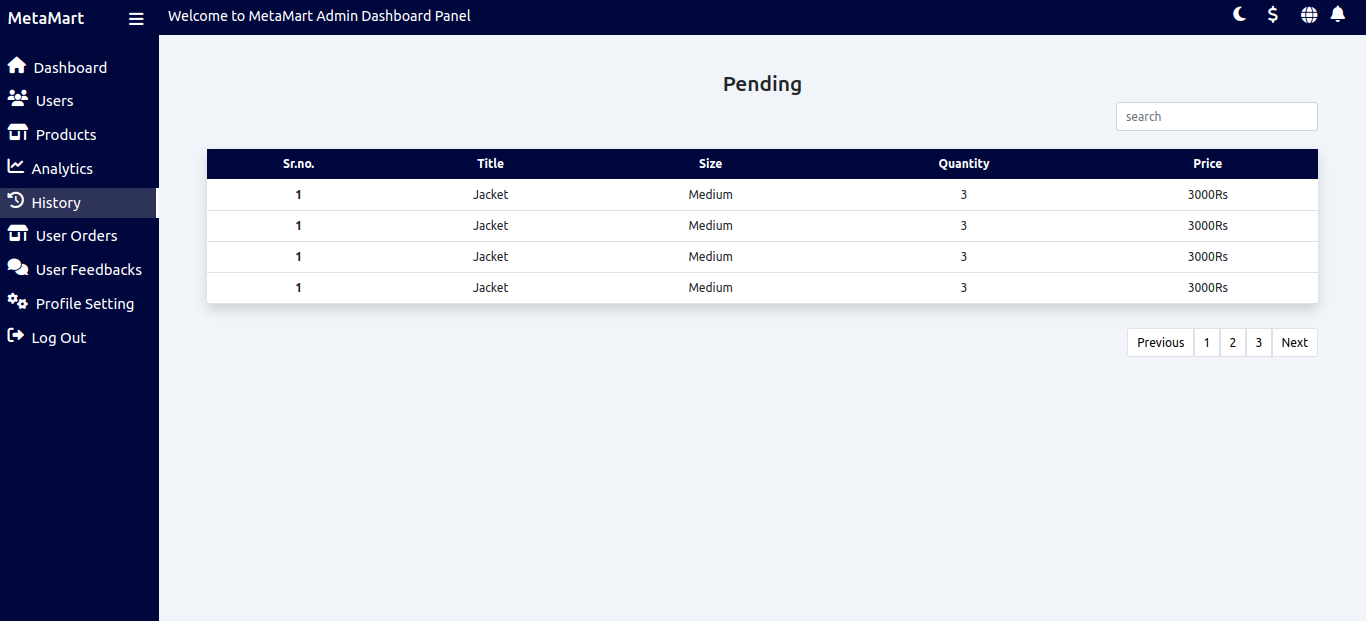
\includegraphics[width=15cm,height=12cm]{Figures/Customer_Section_Images/PendingOrderDetail.png}
    \caption{Admin’s pending orders page}
    \label{Admin’s pending orders page}
\end{figure}
\justifying
This image shows the pending orders screen that we have developed for our MetaMart Application for admin of application. In this screen, there is a table that contains all the orders that are in the queue such that they are not yet received by the customer. Admin can search for an order by order id or simply can explore all orders by next and previous buttons.
\subsection{Customer Section}
\subsubsection{Home Screen}
\begin{figure}[H]
    \centering
    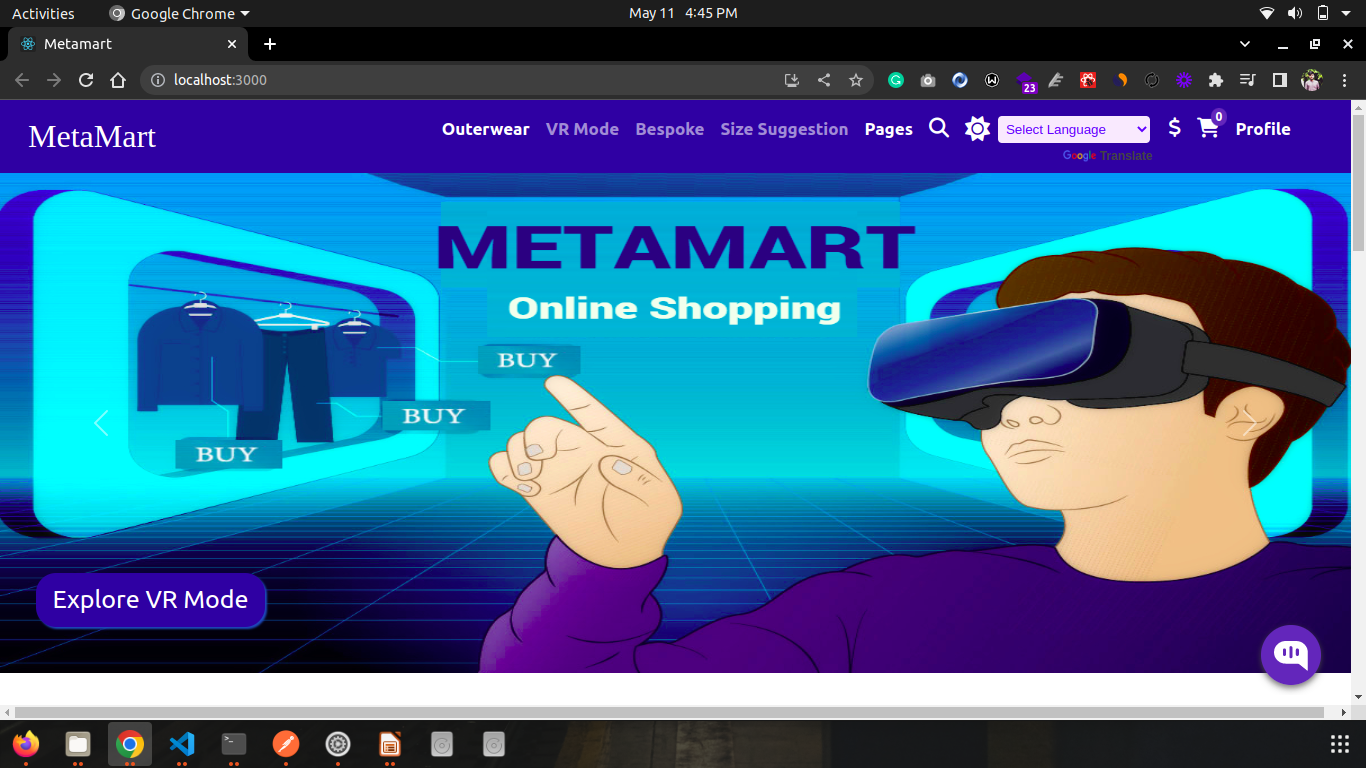
\includegraphics[width=15cm,height=15cm]{Figures/Websites/Customer/customerDashboard.png}
    \caption{Customer’s home page}
    \label{Customer’s home page}
   Home screen for the customer like when the customer will open a virtual reality-based e-commerce web application then this is the main entry point of the website that will be shown to the customer.
\end{figure}
\justifying
This image shows the customer’s home page where the customer would find an option to explore the 3D environment that we have developed for our MetaMart Application. Customers would be able to explore different products just like in the real world.
\subsubsection{Product Section}
\begin{figure}[H]
    \centering
    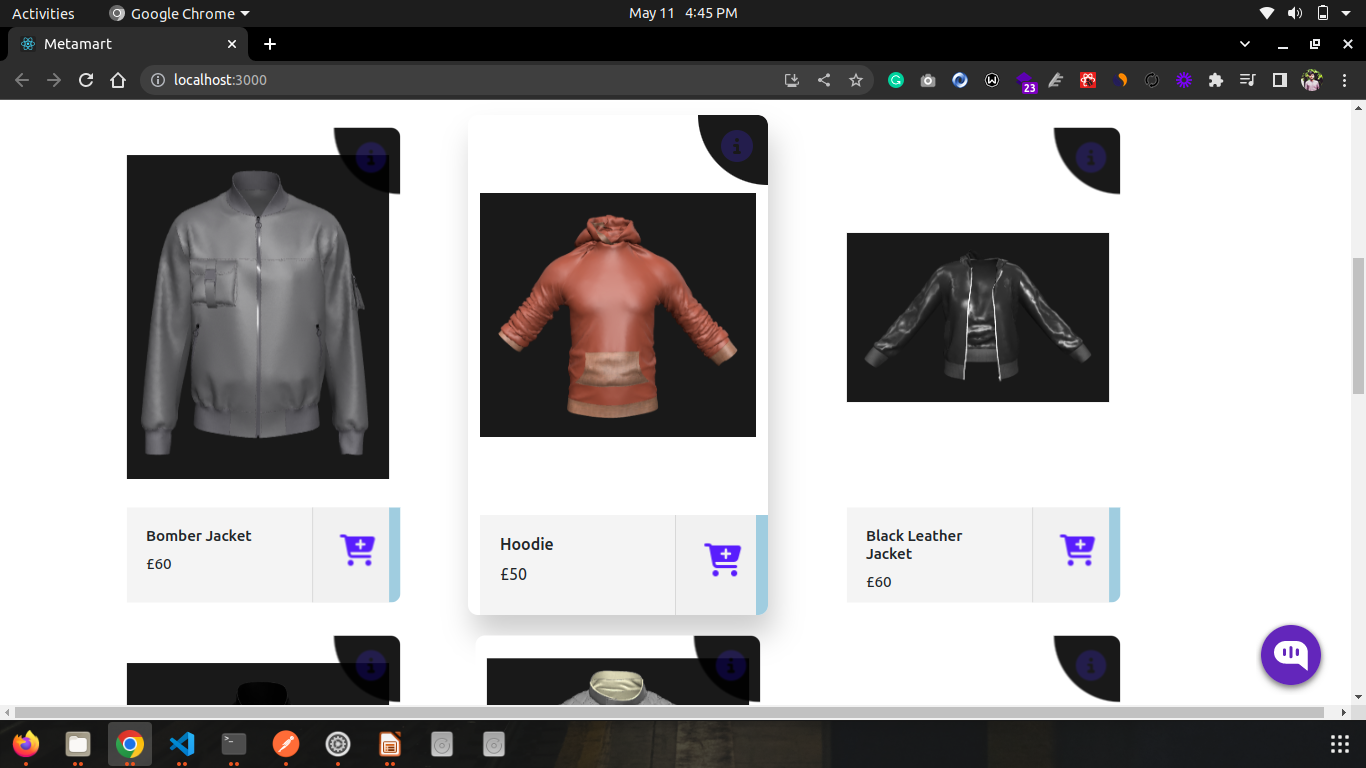
\includegraphics[width=15cm,height=15cm]{Figures/Websites/Customer/CustomerProductList.png}
    \caption{Customer’s products page}
    \label{fig: Product section for customer}
\end{figure}
\justifying
This image shows the customer’s products page where customers would find all products in a general view(2D) just like other e-commerce websites. Here customers can search for a particular product and can see the details of that product by clicking on the details button rendered under every product’s image.
\subsubsection{Signin Section}
\begin{figure}[H]
    \centering
    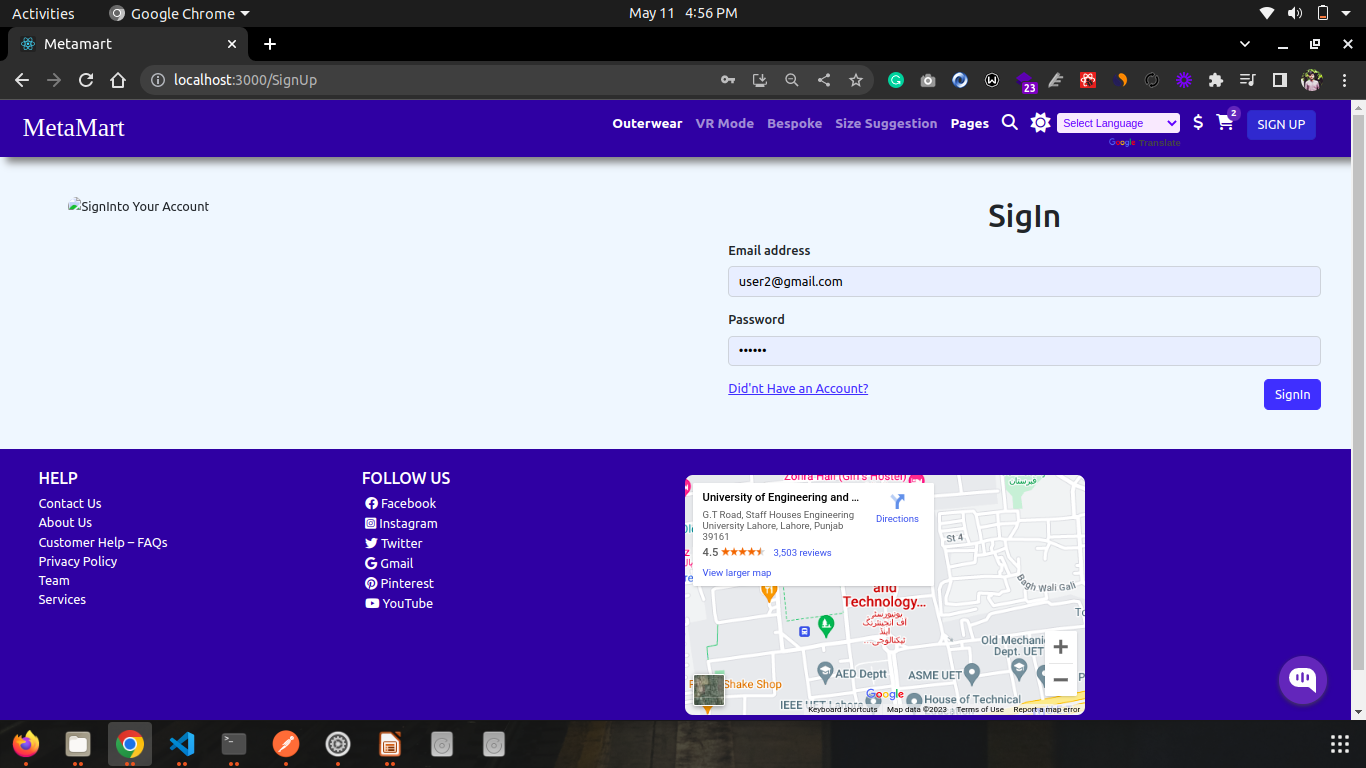
\includegraphics[width=15cm,height=15cm]{Figures/Websites/Customer/CustomerSignin.png}
    \caption{Customer’s products page}
    \label{fig:SignIn Page}
\end{figure}
\justifying

This is the sign-in page where customers can enter their credentials to make a payment for the products they have added to their cart.
\subsubsection{Size suggestion Section}
\begin{figure}[H]
    \centering
    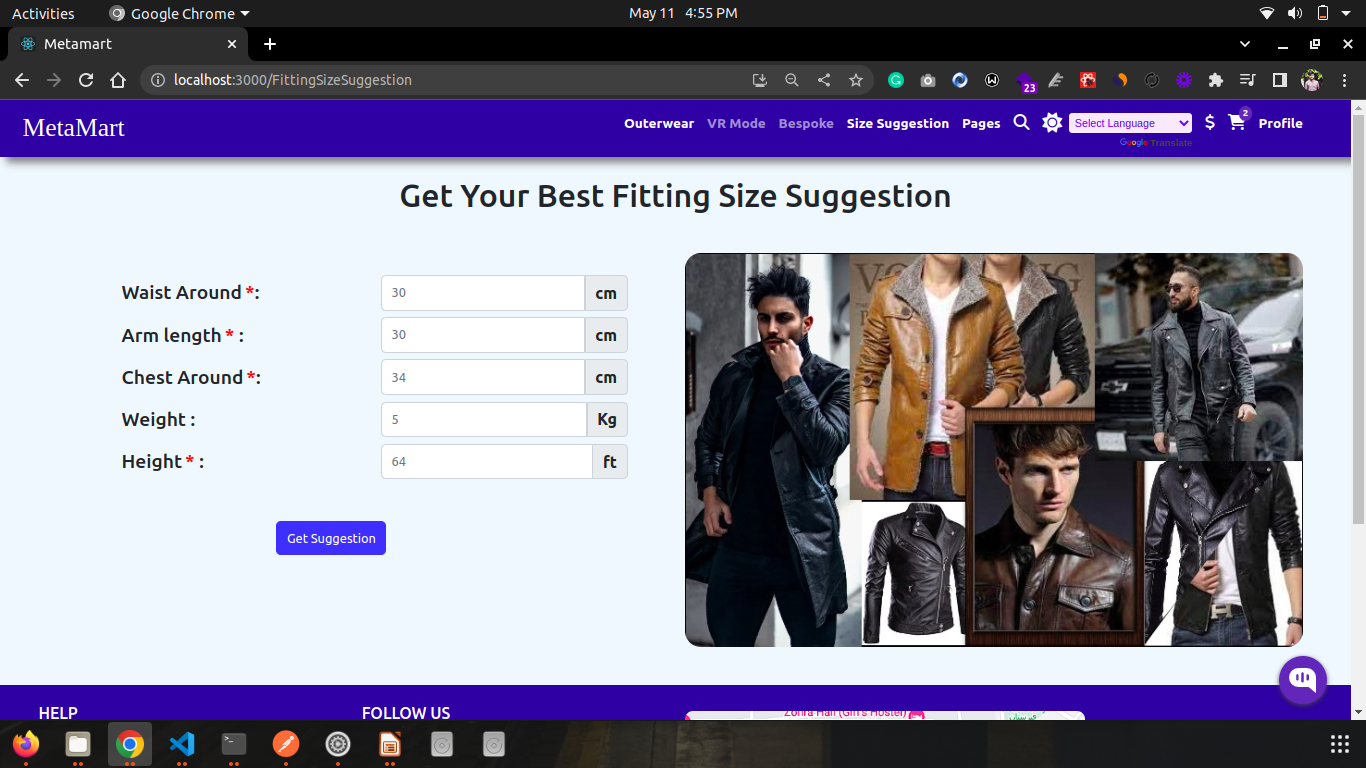
\includegraphics[width=15cm,height=15cm]{Figures/Websites/Customer/CustomerSizeSugestion.png}
    \caption{Customer’s Size suggestion Section}
    \label{fig:Size suggestion Section}
\end{figure}
\justifying

This is the customer size suggestion section.